\documentclass{article}
\usepackage{forest}
\usepackage{amsmath}
\usepackage[margin=1in]{geometry}
\usepackage{tikz}
\usepackage{enumitem}
\usepackage{pdflscape}
\usepackage{amsmath}
\usepackage{amssymb}
\usepackage{float}
\usepackage{array}
\usepackage{longtable}
\usepackage{multirow}
\usepackage[table]{xcolor}
\usepackage{colortbl}
\usetikzlibrary{arrows.meta, positioning, matrix,automata}
\usetikzlibrary{matrix}
\begin{document}
		\author{ Mojtaba Mollaei \\ 40131383 }
	\title{ \huge HW3 }
	\maketitle
\section{}
	\textbf{Expression:} \((4 + 2) * (9 - 3) + 5\)
	
	\textbf{Annotated Parse Tree:}
	
\begin{forest}
	for tree={
		draw, 
		rounded corners,
		edge={->},
		align=center,
		inner sep=2pt,
		parent anchor=south,
		child anchor=north
	}
	[E\\val=41
	[E\\val=36
	[T\\val=36
	[T\\val=6
	[F\\val=6
	[(E)\\val=6
	[E\\val=6
	[E\\val=4
	[T\\val=4
	[F\\val=4
	[digit\\lexval=4]
	]
	]
	]
	[+]
	[T\\val=2
	[F\\val=2
	[digit\\lexval=2]
	]
	]
	]
	]
	]
	]
	[*]
	[F\\val=6
	[(E)\\val=6
	[E\\val=6
	[E\\val=9
	[T\\val=9
	[F\\val=9
	[digit\\lexval=9]
	]
	]
	]
	[-]
	[T\\val=3
	[F\\val=3
	[digit\\lexval=3]
	]
	]
	]
	]
	]
	]
	]
	[+]
	[T\\val=5
	[F\\val=5
	[digit\\lexval=5]
	]
	]
	]
\end{forest}

\textbf{Final Result:} \(E.val = 36 + 5 = \boxed{41}\)
	
	
\section{}

\textbf{Production Rules and Semantic Actions:}

\begin{align*}
	1. \quad & E \rightarrow T\ E' \quad & E'.inh = T.val,\quad E.val = E'.syn \\
	2. \quad & E' \rightarrow +\ T\ E'_1 \quad & E'_1.inh = E'.inh + T.val,\quad E'.syn = E'_1.syn \\
	3. \quad & E' \rightarrow \epsilon \quad & E'.syn = E'.inh \\
	4. \quad & T \rightarrow F\ T' \quad & T'.inh = F.val,\quad T.val = T'.syn \\
	5. \quad & T' \rightarrow *\ F\ T'_1 \quad & T'_1.inh = T'.inh * F.val,\quad T'.syn = T'_1.syn \\
	6. \quad & T' \rightarrow \epsilon \quad & T'.syn = T'.inh \\
	7. \quad & F \rightarrow digit \quad & F.val = digit.lexval
\end{align*}

\bigskip

\textbf{Input String:} $3 + 4 \times 5$

\bigskip

\textbf{Dependency Graph:}



\begin{landscape}
	\begin{center}
		\begin{tikzpicture}[
			every node/.style={
				draw, 
				rounded corners, 
				align=center, 
				minimum width=1cm,
				minimum height=0.7cm,
				font=\tiny,
				inner sep=1pt
			},
			inh/.style={->, red, thick, >=Stealth, shorten >=1pt, shorten <=1pt},
			synth/.style={->, blue, thick, >=Stealth, shorten >=1pt, shorten <=1pt},
			val/.style={->, dashed, gray, thick, >=Stealth, shorten >=1pt, shorten <=1pt}
			]
			
			% Level 1
			\node (E) at (0,0) {E\\E.val};
			
			% Level 2 - much wider spacing
			\node[below left=1.5cm and 3cm of E] (T1) {T\\T.val};
			\node[below right=1.5cm and 4cm of E] (E1) {E'\\E'.inh\\E'.syn};
			
			% Level 3 - left side
			\node[below left=1cm and 1.5cm of T1] (F1) {F\\F.val=3};
			\node[below right=1cm and 1.5cm of T1] (T1p) {T'\\T'.inh\\T'.syn};
			
			% Level 4 (right side) - moved much further right
			\node[below right=5cm and 5cm of E1] (T2) {T\\T.val};
			\node[below right=2cm and 3cm of T2] (E2) {E'\\E'.inh\\E'.syn};
			
			% Level 5 (T2 children) - more spacing
			\node[below left=3cm and 1.5cm of T2] (F2) {F\\F.val=4};
			\node[below right=2cm and 1.5cm of T2] (T2p) {T'\\T'.inh\\T'.syn};
			
			% Level 6 - bottom node with more space
			\node[below=2cm of T2p] (F3) {F\\F.val=5};
			
			% Arrows
			\draw[synth] (F1) -- (T1p) node[pos=0.3, left] {\tiny F.val};
			\draw[inh] (T1p) -- (T1) node[pos=0.3, left] {\tiny T'.syn};
			\draw[synth] (T1) -- (E1) node[pos=0.3, above left] {\tiny T.val};
			\draw[inh] (E1) -- (E) node[pos=0.3, above right] {\tiny E'.syn};
			
			\draw[synth] (F2) -- (T2p) node[pos=0.3, left] {\tiny F.val};
			\draw[synth] (F3) -- (T2p) node[pos=0.3, right] {\tiny F.val};
			\draw[inh] (T2p) -- (T2) node[pos=0.3, right] {\tiny T'.syn};
			\draw[synth] (T2) -- (E2) node[pos=0.3, right] {\tiny T.val};
			\draw[inh] (E2) -- (E1) node[pos=0.3, right] {\tiny E'.syn};
			
			\draw[inh] (E1) -- (E2) node[pos=0.5, above, sloped] {\tiny E'.inh};
			
		\end{tikzpicture}
	\end{center}
\end{landscape}
\bigskip

\textbf{Final Evaluated Values:}

\begin{itemize}
	\item \texttt{F1.val = 3}, \texttt{T'.inh = 3} → \texttt{T.val = 3}
	\item \texttt{F2.val = 4}, \texttt{F3.val = 5}, \texttt{T'.inh = 4}, \texttt{T'.syn = 20} → \texttt{T.val = 20}
	\item \texttt{E'.inh = 3}, \texttt{E'.syn = 3 	+ 20 = 23} → \texttt{E.val = 23}
\end{itemize}
	
	

\section{}



\subsection*{Grammar 1}
\[
\begin{aligned}
	& S \rightarrow A \ B \\
	& A.\text{val} = 1 \\
	& B.\text{inh} = A.\text{val} \\
	& B.\text{val} = B.\text{inh} + 2 \\
\end{aligned}
\]

\textbf{Classification:} L-attributed but not S-attributed

\textbf{Justification:}
\begin{itemize}
	\item \textbf{S-attributed} grammars allow only synthesized attributes. This grammar uses the inherited attribute \texttt{B.inh}, so it is not S-attributed.
	\item \textbf{L-attributed} grammars allow inherited attributes as long as each inherited attribute of a symbol on the right-hand side depends only on:
	\begin{itemize}
		\item The attributes of symbols to its left in the production
		\item The inherited attributes of the head
	\end{itemize}
	Here, \texttt{B.inh} depends on \texttt{A.val}, which is to the left of \texttt{B}, so the grammar is L-attributed.
\end{itemize}

\subsection*{Grammar 2}
\[
\begin{aligned}
	& E \rightarrow E_1 + T \\
	& E.\text{val} = E_1.\text{val} + T.\text{val} \\
	\\
	& E \rightarrow T \\
	& E.\text{val} = T.\text{val} \\
	\\
	& T \rightarrow \text{digit} \\
	& T.\text{val} = \text{digit.lexval}
\end{aligned}
\]

\textbf{Classification:} S-attributed

\textbf{Justification:}
\begin{itemize}
	\item All attributes in the grammar are synthesized:
	\begin{itemize}
		\item \texttt{E.val}, \texttt{T.val} are computed based on the synthesized attributes of their children.
	\end{itemize}
	\item There are no inherited attributes, so this grammar is S-attributed.
	\item Since all S-attributed grammars are also L-attributed, this grammar is also L-attributed.
\end{itemize}

\subsection*{Grammar 3}
\[
\begin{aligned}
	& L \rightarrow L_1 , \ id \\
	& id.\text{pos} = L_1.\text{pos} + 1 \\
	& L.\text{pos} = id.\text{pos} \\
	\\
	& L \rightarrow id \\
	& id.\text{pos} = 1 \\
	& L.\text{pos} = id.\text{pos}
\end{aligned}
\]

\textbf{Classification:} L-attributed but not S-attributed

\textbf{Justification:}
\begin{itemize}
	\item The attribute \texttt{id.pos} is inherited from \texttt{L-1.pos}, so inherited attributes are used.
	\item Since \texttt{id.pos} depends on \texttt{L1.pos}, which is to the left of \texttt{id}, this fits the L-attributed grammar constraints.
	\item The presence of inherited attributes means it is not S-attributed.
\end{itemize}
	
	
\section{}



\subsection*{1. LR($k$)}
\begin{itemize}[leftmargin=*]
	\item \textbf{Power:} Most powerful among the listed methods. Can recognize the largest class of context-free grammars for any fixed $k \geq 1$.
	\item \textbf{Simplicity:} Most complex to implement. Parsing tables grow exponentially with $k$, making it impractical for large $k$. Rarely used in practice beyond $k = 1$.
\end{itemize}

\subsection*{2. LR(1)}
\begin{itemize}[leftmargin=*]
	\item \textbf{Power:} Can handle all deterministic context-free grammars that require only one symbol of lookahead.
	\item \textbf{Simplicity:} More practical than LR($k$) but still generates large parsing tables (many states). Used in some parser generators (e.g., GNU Bison supports canonical LR(1)).
\end{itemize}

\subsection*{3. LALR(1) (Look-Ahead LR)}
\begin{itemize}[leftmargin=*]
	\item \textbf{Power:} Less powerful than full LR(1) but more powerful than SLR(1). Can handle many practical programming language grammars.
	\item \textbf{Simplicity:} Merges LR(1) states with identical cores to reduce table size, making it similar in size to SLR(1) tables. Commonly used in practice (e.g., Yacc, Bison).
\end{itemize}

\subsection*{4. SLR(1) (Simple LR)}
\begin{itemize}[leftmargin=*]
	\item \textbf{Power:} Least powerful among the four. Uses FOLLOW sets for reduce decisions, which may lead to conflicts in some grammars that LR(1) or LALR(1) could handle.
	\item \textbf{Simplicity:} Easiest to implement. Smallest parsing tables. Good for educational purposes and simple languages.
\end{itemize}

\section{}



\subsection*{(a) Grammar}


\textbf{First Sets:}
\begin{align*}
	\text{First}(A) &= \{a, \varepsilon\} \\
	\text{First}(B) &= \{b\} \\
	\text{First}(D) &= \{a, \varepsilon\} \\
	\text{First}(S) &= \{a, b\} \\
	\text{First}(S') &= \{a, b\} \\
\end{align*}

\textbf{Follow Sets:}
\begin{align*}
	\text{Follow}(S) &= \{\$\} \\
	\text{Follow}(A) &= \{b\} \\
	\text{Follow}(B) &= \{d\} \\
	\text{Follow}(D) &= \{\$\}
\end{align*}

\textbf{Canonical LR(1) Items: Initial State \( I_0 \)}

\[
\begin{array}{ll}
	S' \to \cdot S, & \$ \\
	S \to \cdot ABdD, & \$ \\
	S \to \cdot bD, & \$ \\
	A \to \cdot aA, & b \\
	A \to \cdot \varepsilon, & b \\
	B \to \cdot b, & d
\end{array}
\]

\textbf{Conflict in LALR(1) Table:}

After merging LR(1) items with the same LR(0) core, we obtain:

\begin{itemize}
	\item \texttt{A → $\varepsilon$}, lookahead: \{b, d\}
	\item \texttt{B → b}, lookahead: \{d\}
\end{itemize}

On lookahead \texttt{b}, the parser cannot decide whether to:

\begin{itemize}
	\item Reduce using \texttt{A → $\varepsilon$}, or
	\item Shift \texttt{b} to match \texttt{B → b}
\end{itemize}

This results in a \textbf{shift/reduce conflict} in the LALR(1) parsing table.

\textbf{Conclusion:} The grammar is \textbf{not LALR(1)}.

\subsection*{(b) Grammar}

\textbf{First Sets:}
\begin{itemize}
	\item $\text{FIRST}(S) = \{ a, b \}$
	\item $\text{FIRST}(S) = \{ a, b \}$
	\item $\text{FIRST}(A) = \{ a, b \}$
\end{itemize}

\textbf{Follow Sets:}
\begin{itemize}
	\item $\text{FOLLOW}(S') = \{ \$ \}$
	\item $\text{FOLLOW}(S) = \{ \$, \}$
	\item $\text{FOLLOW}(A) = \{ \$, \}$
\end{itemize}

\textbf{state table}

\begin{table}[H]
	\centering
	\begin{tabular}{|c|l|l|l|}
		\hline
		\textbf{State} & \textbf{Kernel} & \textbf{GOTO} & \textbf{Closure} \\
		\hline
		0 & $S' \rightarrow S, \$ $ & & $S' \rightarrow S, \$ $ \\
		& & & $S \rightarrow (A, \$), \$ $ \\
		& & & $A \rightarrow AS, \$ $ \\
		& & & $A \rightarrow .b, \$ $ \\
		\hline
		1 & $S' \rightarrow S., \$ $ & $\text{getc}(G, S)$ & $S' \rightarrow S., \$ $ \\
		\hline
		2 & $S \rightarrow (A, S), \$, $ & $\text{getc}(G, C)$ & $S \rightarrow (A, \$), \$ $ \\
		& & & $A \rightarrow .aS, \$ $ \\
		& & & $A \rightarrow .b, \$ $ \\
		\hline
		3 & $S \rightarrow A., \$, $ & $\text{getc}(G, A)$ & $S \rightarrow A., \$, $ \\
		\hline
		4 & $A \rightarrow a.S, \$, $ & $\text{getc}(G, a)$ & $A \rightarrow .aS, \$, $ \\
		& & & $S \rightarrow (A, \$), \$, $ \\
		& & & $A \rightarrow .aS, \$, $ \\
		& & & $A \rightarrow .b, \$, $ \\
		\hline
		5 & $A \rightarrow b., \$, $ & $\text{getc}(G, b)$ & $A \rightarrow b., \$, $ \\
		\hline
		6 & $S \rightarrow (A., S), \$, $ & $\text{getc}(2, A)$ & $S \rightarrow (A., \$), \$, $ \\
		\hline
		4 & $A \rightarrow a.S, \$, $ & $\text{gotc}(2, a)$ & \\
		\hline
		5 & $A \rightarrow b. \$, $ & $\text{getc}(2, b)$ & \\
		\hline
		7 & $S \rightarrow aS., \$, $ & $\text{getc}(G, S)$ & $A \rightarrow aS., \$, $ \\
		\hline
		4 & $\{A \rightarrow a.A, b\}$ & $\text{getc}(G, a)$ & \\
		\hline
		2 & $S \rightarrow (A, S), \$, $ & $\text{getc}(G, C)$ & \\
		\hline
		3 & $S \rightarrow A., \$, $ & $\text{getc}(G, A)$ & \\
		\hline
		4 & & $\text{getc}(G, a)$ & \\
		\hline
		5 & & $\text{getc}(G, b)$ & \\

\hline
8 & $S = (A, .S), \$$ & $\text{getc}(6, .)$ & $A = .aS, 0, S = (A, .S), \$$ \\
& & & $S = (A, .S), 0, S = .A, 0, A = .aS, 0, A = .b, 0$ \\
\hline
9 & $S = (A, .S), \$$ & $\text{getc}(8, .S)$ & $S = (A, .S), \$$ \\
\hline
2 & $S = (A, .S), \$$ & $\text{getc}(8, .C)$ & \\
\hline
3 & $S = A, .\$$ & $\text{getc}(8, .A)$ & \\
\hline
4 & $S = a.S, \$$ & $\text{getc}(8, .a)$ & \\
\hline
5 & $S = b., \$$ & $\text{getc}(8, .b)$ & \\
\hline
10 & $S = (A, .S), \$$ & $\text{getc}(9, .)$ & $S = (A, .S), \$$ \\
\hline

	\end{tabular}
	
\end{table}

\textbf{Parsing table}

\begin{table}[H]
	\centering
	\begin{tabular}{|c|c|c|c|c|c|c|c|}
		\hline
		\textbf{State} & \textbf{(} & \textbf{)} & \textbf{a} & \textbf{b} & \textbf{\$} & \textbf{S} & \textbf{A} \\
		\hline
		0 & s2 & & s4 & s5 & -1 & 1 & 3 \\
		\hline
		1 & & & & & \text{accept} & & \\
		\hline
		2 & & & s4 & s5 & -1 & 6 & \\
		\hline
		3 & r2 & r2 & & -1 & r2 & & \\
		\hline
		4 & s2 & & s4 & s5 & -7 & 7 & 3 \\
		\hline
		5 & r4 & r4 & & -1 & r4 & & \\
		\hline
		6 & s8 & & & & & & \\
		\hline
		7 & r3 & r3 & & -1 & r3 & & \\
		\hline
		8 & s2 & & s4 & s5 & -9 & 9 & 3 \\
		\hline
		9 & & s10 & & & & & \\
		\hline
		10 & r1 & r1 & & -1 & r1 & & \\
		\hline
	\end{tabular}
\end{table}

\section{}


\begin{enumerate}
	\item $S \rightarrow ABC$
	\item $A \rightarrow aqA$
	\item $A \rightarrow \varepsilon$
	\item $B \rightarrow bBqA$
	\item $B \rightarrow \varepsilon$
	\item $C \rightarrow cC$
	\item $C \rightarrow \varepsilon$
\end{enumerate}



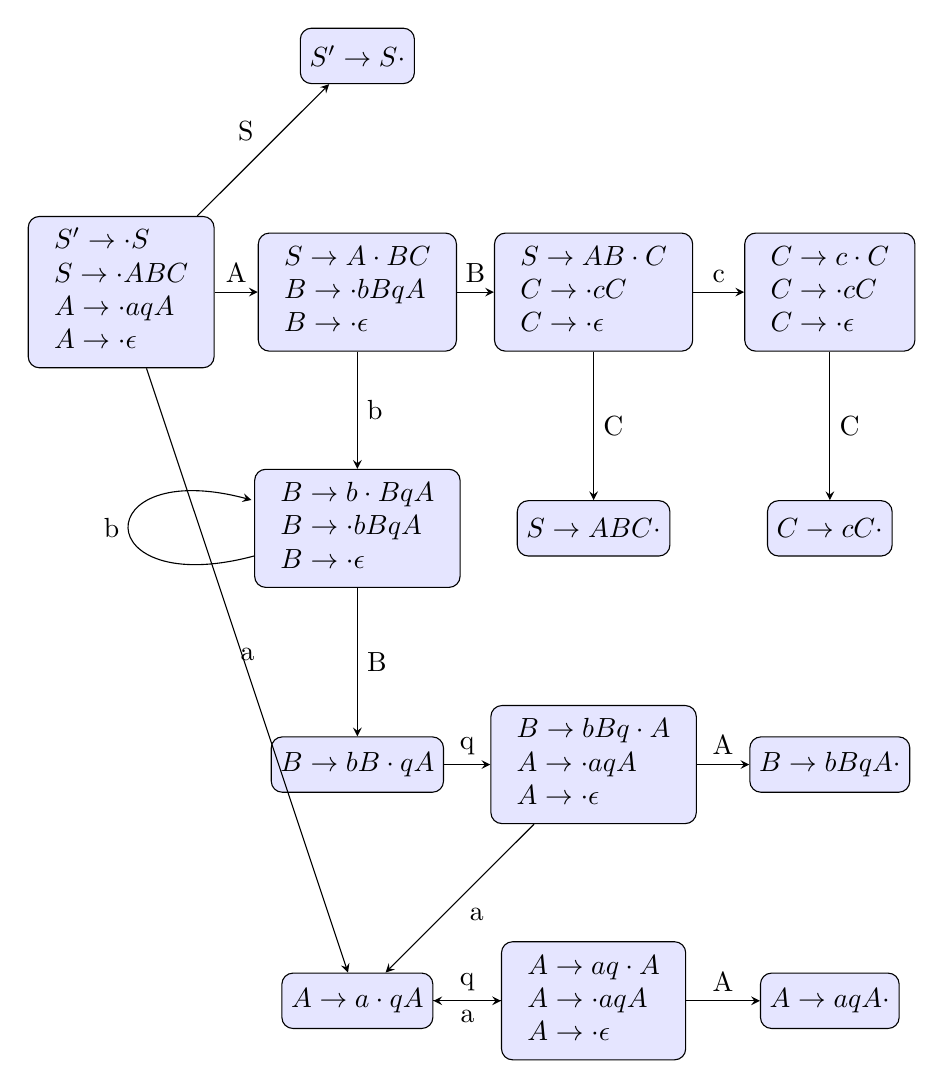
\begin{tikzpicture}[node distance=3cm and 3cm, on grid, auto,
	  state/.style={rectangle, draw, rounded corners, minimum height=2em, minimum width=2em, fill=blue!10},
	final/.style={ellipse, draw, fill=yellow!30},
	->, >=stealth]

% Nodes
\node[state] (I0) at (0,0) {%
	\begin{tabular}{l}
		$S' \rightarrow \cdot S$\\
		$S \rightarrow \cdot ABC$\\
		$A \rightarrow \cdot aqA$\\
		$A \rightarrow \cdot \epsilon$
	\end{tabular}
};

\node[state, above right=of I0] (I1) {$S' \rightarrow S\cdot$};
\node[state, right=of I0] (I2) {%
	\begin{tabular}{l}
		$S \rightarrow A\cdot BC$\\
		$B \rightarrow \cdot bBqA$\\
		$B \rightarrow \cdot \epsilon$
	\end{tabular}
};

\node[state, right=of I2] (I4) {%
	\begin{tabular}{l}
		$S \rightarrow AB\cdot C$\\
		$C \rightarrow \cdot cC$\\
		$C \rightarrow \cdot \epsilon$
	\end{tabular}
};

\node[state, right=of I4] (I8) {%
	\begin{tabular}{l}
		$C \rightarrow c\cdot C$\\
		$C \rightarrow \cdot cC$\\
		$C \rightarrow \cdot \epsilon$
	\end{tabular}
};

\node[state, below=of I8] (I11) {$C \rightarrow cC\cdot$};

\node[state, below=of I4] (I7) {$S \rightarrow ABC\cdot$};

\node[state, below=of I2] (I5) {%
	\begin{tabular}{l}
		$B \rightarrow b\cdot BqA$\\
		$B \rightarrow \cdot bBqA$\\
		$B \rightarrow \cdot \epsilon$
	\end{tabular}
};

\node[state, below=of I5] (I9) {$B \rightarrow bB\cdot qA$};

\node[state, right=of I9] (I12) {%
	\begin{tabular}{l}
		$B \rightarrow bBq\cdot A$\\
		$A \rightarrow \cdot aqA$\\
		$A \rightarrow \cdot \epsilon$
	\end{tabular}
};

\node[state, right=of I12] (I13) {$B \rightarrow bBqA\cdot$};

\node[state, below left=of I12] (I3) {$A \rightarrow a\cdot qA$};
\node[state, right=of I3] (I6) {%
	\begin{tabular}{l}
		$A \rightarrow aq\cdot A$\\
		$A \rightarrow \cdot aqA$\\
		$A \rightarrow \cdot \epsilon$
	\end{tabular}
};

\node[state, right=of I6] (I10) {$A \rightarrow aqA\cdot$};
%\node[final, below right=of I5] (I3accept) {I3};

% Transitions
\draw (I0) -- node {S} (I1);
\draw (I0) -- node {A} (I2);
\draw (I0) -- node[above] {a} (I3);
\draw (I3) -- node {q} (I6);
\draw (I6) -- node {A} (I10);
\draw (I2) -- node {B} (I4);
\draw (I4) -- node {C} (I7);
\draw (I4) -- node {c} (I8);
\draw (I8) -- node {C} (I11);
\draw (I2) -- node {b} (I5);
\draw (I5) edge[loop left] node {b} ();
\draw (I5) -- node {B} (I9);
\draw (I9) -- node {q} (I12);
\draw (I12) -- node {A} (I13);
\draw (I6) --   node [bend left] {a} (I3);
\draw (I12) --   node [bend left] {a} (I3);
\end{tikzpicture}


\begin{table}[H]
	\centering
	\renewcommand{\arraystretch}{1.2}
	\setlength{\tabcolsep}{8pt}
	
	\begin{tabular}{|c||>{\columncolor{blue!20}}c|>{\columncolor{blue!20}}c|>{\columncolor{blue!20}}c|>{\columncolor{blue!20}}c|>{\columncolor{blue!20}}c|>{\columncolor{green!20}}c|>{\columncolor{green!20}}c|>{\columncolor{green!20}}c|>{\columncolor{green!20}}c|}
		\hline
		\textbf{State} & \textbf{a} & \textbf{b} & \textbf{c} & \textbf{q} & \textbf{\$} & \textbf{S} & \textbf{A} & \textbf{B} & \textbf{C} \\
		\hline
		0  & s3  & r3  & r3  & r3  & r3  & 1 & 2 &   &   \\
		1  &     &     &     &     & accept &   &   &   &   \\
		2  &     & s5  &  r5 & r5  &  r5 &   &   & 4  &   \\
		3  &     &     &     &  s6 &     &   &   &    &   \\
		4  &     &     &  s8 &     & r7  &   &   &   & 7 \\
		5  &     & s5  & r5  & r5  & r5  &   &   & 9 &   \\
		6  & s3  & r3  & r3  & r3  & r3  &   &10 &   &   \\
		7  &     &     &     &     & r1  &   &   &   &   \\
		8  &     &     & s8  &     & r7  &   &   &   & 11 \\
		9  &     &     &     & s12 &     &   &   &   &   \\
		10 &     & r2  & r2  & r2  & r2  &   &   &   &   \\
		11 &     &     &     &     & r6  &   &   &   &   \\
		12 & s3  & r3  & r3  & r3  & r3  &   &13 &   &   \\
		13 &     & r4  &  r4 & r4  &     &   &   &   &   \\
		\hline
	\end{tabular}
\end{table}
\begin{table}[H]
	\centering
	\begin{tabular}{|c|c|c|c|}
		\hline
		\textbf{Step} & \textbf{Stack} & \textbf{Input} & \textbf{Action} \\ \hline
		1 & 0 & aqbqcc\$ & s3 \\ \hline
		2 & 0a3 & qbqcc\$ & s6 \\ \hline
		3 & 0a3q6 & bqcc\$ & r3 \\ \hline
		4 & 0a3q6A10 & bqcc\$ & r2 \\ \hline
		5 & 0A2 & bqcc\$ & s5 \\ \hline
		6 & 0A2b5 & qcc\$ & r5 \\ \hline
		7 & 0A2b5B9 & qcc\$ & s12 \\ \hline
		8 & 0A2b5B9q12 & cc\$ & r3 \\ \hline
		9 & 0A2b5B9q12A13 & cc\$ & s8 \\ \hline
		10 & 0A2B4 & cc\$ & s8 \\ \hline
		11 & 0A2B4c8 & c\$ & s8 \\ \hline
		12 & 0A2B4c8c8 & \$ & r7 \\ \hline
		13 & 0A2B4c8c8C11 & \$ & r6 \\ \hline
		14 & 0A2B4c8C11 & \$ & r6 \\ \hline
		15 & 0A2B4C7 & \$ & r1 \\ \hline
		16 & 0S1 & \$ & Accept \\ \hline
	\end{tabular}
\end{table}

\section{}

\begin{itemize}
	\item \textbf{S0} \\
	$[S' \rightarrow \cdot S, S]$ \\
	$[S \rightarrow \cdot XdY, S]$ \\
	$[X \rightarrow \cdot aX, d]$ \\
	$[X \rightarrow \cdot \epsilon, d]$
	
	\item \textbf{S1} \\
	$[S' \rightarrow S \cdot, S]$
	
	\item \textbf{S2} \\
	$[S \rightarrow X \cdot dY, S]$
	
	\item \textbf{S3} \\
	$[X \rightarrow a \cdot X, d]$ \\
	$[X \rightarrow \cdot aX, d]$ \\
	$[X \rightarrow \cdot \epsilon, d]$
	
	\item \textbf{S5} \\
	$[X \rightarrow aX \cdot, d]$
	
	\item \textbf{S9} \\
	$[Y \rightarrow bY \cdot S, S]$ \\
	$[S \rightarrow \cdot XdY, S]$ \\
	$[X \rightarrow \cdot aX, d]$ \\
	$[X \rightarrow \cdot \epsilon, d]$
	
	\item \textbf{S10} \\
	$[Y \rightarrow bYS \cdot, S]$
	
	\item \textbf{S12} \\
	$[Y \rightarrow bYS \cdot, a]$
	
	\item \textbf{S13} \\
	$[S \rightarrow X \cdot dY, a/d]$
	
	\item \textbf{S14} \\
	$[Y \rightarrow \cdot bYS, a/d]$ \\
	$[Y \rightarrow \cdot \epsilon, a/d]$
	
	\item \textbf{S15} \\
	$[S \rightarrow XdY \cdot, a/d]$
\end{itemize}


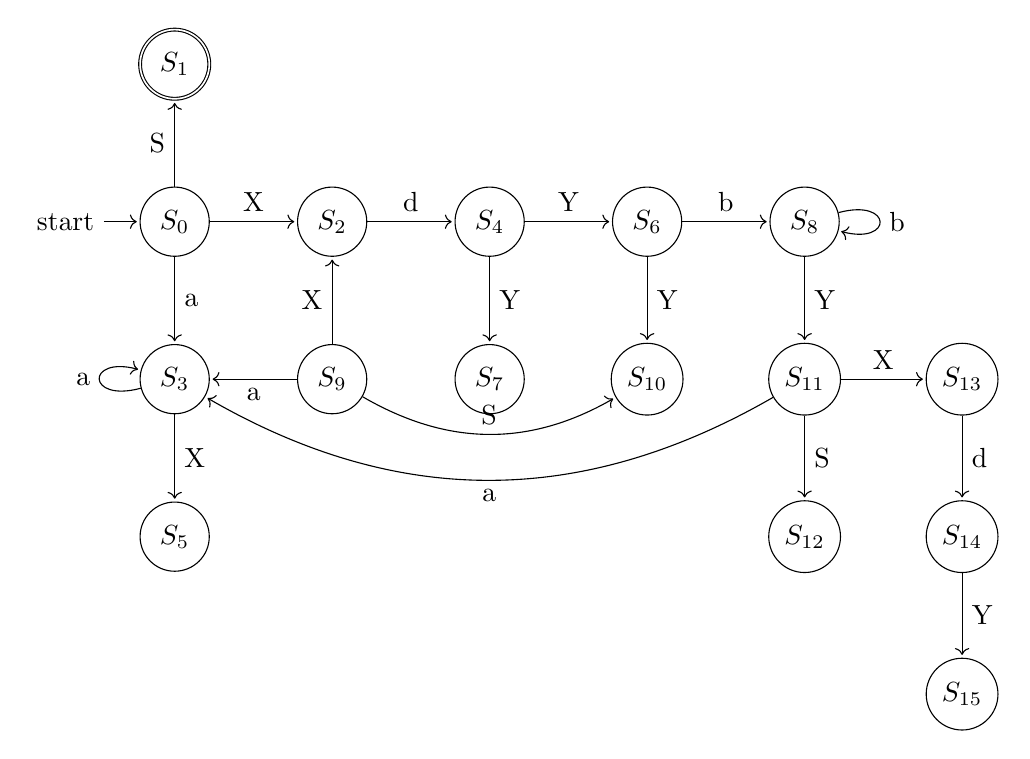
\begin{tikzpicture}[shorten >=1pt, node distance=2cm, on grid, auto]
	\node[state, initial] (S0) {$S_0$};
	\node[state, right=of S0] (S2) {$S_2$};
	\node[state, below=of S0] (S3) {$S_3$};
	\node[state, below=of S3] (S5) {$S_5$};
	\node[state, right=of S2] (S4) {$S_4$};
	\node[state, right=of S4] (S6) {$S_6$};
	\node[state, right=of S6] (S8) {$S_8$};
	\node[state, below=of S4] (S7) {$S_7$};
	\node[state, below=of S6] (S10) {$S_{10}$};
	\node[state, below=of S8] (S11) {$S_{11}$};
	\node[state, below=of S11] (S12) {$S_{12}$};
	\node[state, right=of S11] (S13) {$S_{13}$};
	\node[state, below=of S13] (S14) {$S_{14}$};
	\node[state, below=of S14] (S15) {$S_{15}$};
	\node[state, right=of S3] (S9) {$S_9$};
	\node[state, accepting, above=of S0] (S1) {$S_1$};
	
	% Transitions
	\path[->]
	(S0) edge node {S} (S1)
	edge node {a} (S3)
	edge node {X} (S2)
	(S3) edge[loop left] node {a} ()
	edge node {X} (S5)
	(S2) edge node {d} (S4)
	(S4) edge node {Y} (S7)
	(S4) edge node {Y} (S6)
	(S6) edge node {b} (S8)
	(S6) edge node {Y} (S10)
	(S8) edge[loop right] node {b} ()
	edge node {Y} (S11)
	(S11) edge node {S} (S12)
	(S11) edge[bend left] node {a} (S3)
	%(S12) edge node {S} (S1)
	(S11) edge node {X} (S13)
	(S13) edge node {d} (S14)
	(S14) edge node {Y} (S15)
	(S9) edge node {X} (S2)
	edge node {a} (S3)
	edge[bend right] node {S} (S10)
	;
	
	% You can keep adding more transitions and nodes based on the image.
\end{tikzpicture}

\begin{table}[H]
	\centering

	\begin{tabular}{|c|cccc|ccc|}
		\hline
		\multirow{2}{*}{state} & \multicolumn{4}{c|}{ACTION} & \multicolumn{3}{c|}{GOTO} \\ \cline{2-8}
		& a & b & d & \$ & S & X & Y \\ \hline
		0 & s3 &   & r3 &   & 1 & 2 &   \\ \hline
		1 &   &   &   & accept &   &   &   \\ \hline
		2 &   &   & s4 &   &   &   &   \\ \hline
		3 & s3 &   & r3 &   &   & 5 &   \\ \hline
		4 &   & s6 &   & r5 &   &   & 7 \\ \hline
		5 &   &   & r2 &   &   &   &   \\ \hline
		6 & r5 & s8 &   & r5 &   &   & 9 \\ \hline
		7 &   &   &   & r1 &   &   &   \\ \hline
		8 & r5 & s8 &   & r5 &   &   & 11 \\ \hline
		9 & s3 &   & r3 &   & 10 & 2 &   \\ \hline
		10 &   &   &   & r4 &   &   &   \\ \hline
		11 & s3 &   & r3 &   & 12 & 13 &   \\ \hline
		12 & r4 &   & r4 &   &   &   &   \\ \hline
		13 &   &   & s14 &   &   &   &   \\ \hline
		14 & r5 & s8 & r5  &   &   &   & 15 \\ \hline
		15 & r1 &   & r1 &   &   &   &   \\ \hline
	\end{tabular}
\end{table}
\begin{table}[H]
	\centering
	\caption{LR Parsing Steps for Input String "aadbbadd\$"}
	\begin{tabular}{|c|l|l|l|}
		\hline
		\textbf{Step} & \textbf{Stack} & \textbf{Input} & \textbf{Action} \\ \hline
		1 & 0 & aadbbadd\$ & s3 \\ \hline
		2 & 0a3 & adbbadd\$ & s3 \\ \hline
		3 & 0a3a3 & dbbadd\$ & r3 \\ \hline
		4 & 0a3a3 & dbbadd\$ & Goto X, state 5 \\ \hline
		5 & 0a3a3X5 & dbbadd\$ & r2 \\ \hline
		6 & 0a3 & dbbadd\$ & Goto X, state 5 \\ \hline
		7 & 0a3X5 & dbbadd\$ & r2 \\ \hline
		8 & 0 & dbbadd\$ & Goto X, state 2 \\ \hline
		9 & 0X2 & dbbadd\$ & s4 \\ \hline
		10 & 0X2d4 & bbadd\$ & s6 \\ \hline
		11 & 0X2d4b6 & badd\$ & s8 \\ \hline
		12 & 0X2d4b6b8 & add\$ & r5 \\ \hline
		13 & 0X2d4b6b8 & add\$ & Goto Y, state 11 \\ \hline
		14 & 0X2d4b6b8Y11 & add\$ & s3 \\ \hline
		15 & 0X2d4b6b8Y11a3 & dd\$ & r3 \\ \hline
		16 & 0X2d4b6b8Y11a3 & dd\$ & Goto X, state 13 \\ \hline
		17 & 0X2d4b6b8Y11X13 & dd\$ & s14 \\ \hline
		18 & 0X2d4b6b8Y11X13d14 & d\$ & r5 \\ \hline
		19 & 0X2d4b6b8Y11X13d14 & d\$ & Goto Y, state 15 \\ \hline
		20 & 0X2d4b6b8Y11X13d14Y15 & d\$ & r1 \\ \hline
		21 & 0X2d4b6b8Y11 & d\$ & s12 \\ \hline
		22 & 0X2d4b6b8Y11S12 & d\$ & r4 \\ \hline
		23 & 0X2d4b6 & d\$ & s9 \\ \hline
		24 & 0X2d4b6Y9 & d\$ & r4 \\ \hline
		25 & 0X2d4 & d\$ & s7 \\ \hline
		26 & 0X2d4Y7 & d\$ & r1 \\ \hline
		27 & 0 & d\$ & Goto S, state 1 \\ \hline
		28 & 0S1 & \$ & Accept \\ \hline
	\end{tabular}
\end{table}


\section{}


\begin{itemize}
	\item \textbf{I0} \\
	$[S' \rightarrow \cdot S, \$]$ \\
	$[S \rightarrow \cdot Aa, \$]$ \\
	$[S \rightarrow \cdot bAc, \$]$ \\
	$[S \rightarrow \cdot Bc, \$]$ \\
	$[S \rightarrow \cdot bBa, \$]$ \\
	$[A \rightarrow \cdot d, a]$ \\
	$[B \rightarrow \cdot d, c]$ \\
	
	\item \textbf{I1} \\
	$[S' \rightarrow S\cdot, \$]$ \\
	
	\item \textbf{I2} \\
	$[S \rightarrow A\cdot a, \$]$ \\
	
	\item \textbf{I3} \\
	$[S \rightarrow b\cdot Ac, \$]$ \\
	$[S \rightarrow b\cdot Ba, \$]$ \\
	$[A \rightarrow \cdot d, c]$ \\
	$[B \rightarrow \cdot d, a]$ \\
	
	\item \textbf{I4} \\
	$[S \rightarrow B\cdot c, \$]$ \\
	
	\item \textbf{I5} \\
	$[A \rightarrow d\cdot, a]$ \\
	$[B \rightarrow d\cdot, c]$ \\
	
	\item \textbf{I6} \\
	$[S \rightarrow Aa\cdot, \$]$ \\
	
	\item \textbf{I7} \\
	$[S \rightarrow bA\cdot c, \$]$ \\
	
	\item \textbf{I8} \\
	$[S \rightarrow bB\cdot a, \$]$ \\
	
	\item \textbf{I9} \\
	$[A \rightarrow d\cdot, c]$ \\
	$[B \rightarrow d\cdot, a]$ \\
	
	\item \textbf{I10} \\
	$[S \rightarrow Bc\cdot, \$]$ \\
	
	\item \textbf{I11} \\
	$[S \rightarrow bAc\cdot, \$]$ \\
	
	\item \textbf{I12} \\
	$[S \rightarrow bBa\cdot, \$]$ \\
\end{itemize}

\begin{tikzpicture}[->, >=stealth, shorten >=1pt, auto, node distance=2.5cm, semithick]
	
	% States
	\node[state] (I0) {I0};
	\node[state, above left of=I0, node distance=3cm] (I1) {I1};
	\node[state, above right of=I0] (I2) {I2};
	\node[state, below right of=I0] (I3) {I3};
	\node[state, below of=I0	] (I5) {I5};
	\node[state, above of=I2] (I6) {I6};
	\node[state, right of=I3, node distance=3cm] (I7) {I7};
	\node[state, below of=I7] (I9) {I9};
	\node[state, right of=I7] (I11) {I11};
	\node[state, right of=I2, node distance=3cm] (I4) {I4};
	\node[state, right of=I4] (I10) {I10};
	\node[state, below of=I3, node distance=3.5cm] (I8) {I8};
	\node[state, below of=I8] (I12) {I12};
	
	% Edges
	\path (I1) edge node {S} (I0);
	\path (I0) edge node {A} (I2);
	\path (I0) edge node {b} (I3);
	\path (I0) edge node {B} (I4);
	\path (I0) edge node {d} (I5);
	\path (I2) edge node {a} (I6);
	\path (I3) edge node {A} (I7);
	\path (I3) edge node {d} (I9);
	\path (I3) edge node {B} (I8);
	\path (I4) edge node {c} (I10);
	\path (I7) edge node {c} (I11);
	\path (I8) edge node {a} (I12);
	
\end{tikzpicture}

\begin{table}[H]
	\centering
	\caption{LR(1) Parsing Table}
	\begin{tabular}{|c|*{5}{c|}*{3}{c|}}
		\hline
		State & \multicolumn{5}{c|}{ACTION} & \multicolumn{3}{c|}{GOTO} \\
		\cline{2-9}
		& a & b & c & d & \$ & S & A & B \\
		\hline
		0 &   & s3 &   & s5 &   & 1 & 2 & 4 \\
		1 &   &   &   &  &  accept &   &   &   \\
		2 & s6 &   &   &   &   &   &   &   \\
		3 &   &   &   & s9 &   &   & 7 & 8 \\
		4 &   &   & s10 &   &   &   &   &   \\
		5 & r6 &   & r7 &   &   &   &   &   \\
		6 &   &   &   &   & r2 &   &   &   \\
		7 &   &   & s11 &   &   &   &   &   \\
		8 & s12 &   &   &   &   &   &   &   \\
		9 & r7 &   & r6 &   &   &   &   &   \\
		10 &   &   &   &   & r4 &   &   &   \\
		11 &   &   &   &   & r3 &   &   &   \\
		12 &   &   &   &   & r5 &   &   &   \\
		\hline
	\end{tabular}
\end{table}
\vspace{1cm}

There is no conflict, and as a result, there is no problem for being an LR(1) parser.

Now, to examine conflicts in LALR(1), we need to follow the core shared items. Here, states 5 and 9 share the same core. If we merge them:


\begin{table}[H]
	\centering
	\caption{LALR(1) Parsing Table}
	\begin{tabular}{|c|*{5}{c|}*{3}{c|}}
		\hline
		State & \multicolumn{5}{c|}{ACTION} & \multicolumn{3}{c|}{GOTO} \\
		\cline{2-9}
		& a & b & c & d & \$ & S & A & B \\
		\hline
		0 &   & s3 &   & s5 &   & 1 & 2 & 4 \\
		1 &   &   &   &   &  accept &   &   &   \\
		2 & s6 &   &   &   &   &   &   &   \\
		3 &   &   &   & s9 &   &   & 7 & 8 \\
		4 &   &   & s10 &   &   &   &   &   \\
		\multirow{2}{*}{5,9} & r6/r7 &   & r6/r7 &   &   &   &   &   \\
		& & & & & & & & \\
		6 &   &   &   &   & r2 &   &   &   \\
		7 &   &   & s11 &   &   &   &   &   \\
		8 & s12 &   &   &   &   &   &   &   \\
		10 &   &   &   &   & r4 &   &   &   \\
		11 &   &   &   &   & r3 &   &   &   \\
		12 &   &   &   &   & r5 &   &   &   \\
		\hline
	\end{tabular}
\end{table}
So as we have conflicts here, this is not grammar is not LALR(1).
\end{document}
